\documentclass[12pt,a4paper]{article}
\usepackage[utf8]{inputenc}
\usepackage{geometry}
\usepackage{graphicx}
\usepackage{amsmath}
\usepackage{hyperref}
\usepackage{lipsum}

% Page layout
\geometry{top=1in, bottom=1in, left=1in, right=1in}

% Title settings
\title{\textbf{Deep Learning Course \\ Final Project Report}}
\author{Muhammad Ardiansyah Asrifah (H071221068)\\ Muhammad Azka Sufirman Rahman (H071221032) \\ Mahendra 
Kirana M. B. (H071221058)}
\date{\today}

\begin{document}

\maketitle
\tableofcontents
\newpage

% 1. Introduction
\section{Introduction}
Perkembangan pesat teknologi Deep Learning telah membawa dampak signifikan dalam berbagai bidang, termasuk analisis citra di industri kecantikan. Salah satu area yang menarik adalah pengenalan dan klasifikasi jenis rambut berdasarkan data visual yang beragam, seperti rambut lurus, keriting, atau bergelombang. Rambut memiliki karakteristik unik yang dapat dilihat dari pola, tekstur, dan kerapatan helai, sehingga membedakan jenis rambut secara otomatis memerlukan algoritma canggih. Dalam hal ini, Deep Learning menawarkan pendekatan yang lebih akurat dibandingkan metode tradisional karena kemampuannya dalam mengenali pola kompleks secara otomatis tanpa intervensi manual yang intensif. Masalah utama yang dihadapi dalam proyek ini adalah mengembangkan model Deep Learning yang mampu mengklasifikasikan jenis rambut dari gambar dengan presisi tinggi. Tantangan tambahan adalah memastikan model dapat bekerja secara konsisten pada dataset yang bervariasi, yang mencakup rambut dengan berbagai warna, panjang, dan kondisi pencahayaan. Selain itu, proyek ini juga bertujuan memberikan rekomendasi model rambut yang sesuai berdasarkan jenis rambut yang teridentifikasi, misalnya menyarankan potongan rambut pendek untuk rambut keriting yang tebal atau gaya rambut lurus panjang untuk rambut tipis. Tujuan dari penelitian ini mencakup beberapa aspek penting. Pertama, mengembangkan model klasifikasi yang mampu mengenali perbedaan antara rambut lurus, keriting, dan jenis lainnya dengan tingkat akurasi yang tinggi. Kedua, menciptakan sistem rekomendasi personalisasi yang memberikan saran gaya rambut berdasarkan hasil klasifikasi, sehingga pengguna dapat memilih gaya rambut yang sesuai dengan karakteristik alami rambut mereka. Proyek ini memiliki nilai signifikan dalam bidang Deep Learning karena menawarkan aplikasi nyata yang dapat memberikan manfaat praktis di industri kecantikan dan gaya hidup. Selain itu, penelitian ini berkontribusi pada pengembangan algoritma pengenalan pola yang lebih efektif dalam menangani dataset visual yang kompleks dan bervariasi. Dengan solusi ini, personalisasi dalam pemilihan gaya rambut akan lebih mudah diakses, yang pada akhirnya dapat meningkatkan kepercayaan diri pengguna serta memperluas penerapan teknologi kecerdasan buatan dalam kehidupan sehari-hari.


% 2. Related Works
\section{Related Works}
Berbagai penelitian sebelumnya telah menunjukkan efektivitas Deep Learning dalam klasifikasi gambar, termasuk dalam domain klasifikasi rambut. Studi oleh He et al. (2023) dalam makalah "Image Classification via Residual Networks" menyoroti kemampuan ResNet untuk mengatasi masalah vanishing gradient melalui skip connections, sehingga menghasilkan akurasi yang stabil meskipun menggunakan jaringan dalam. Penelitian lain yang dipublikasikan di Jurnal PTIIK Universitas Brawijaya menggunakan arsitektur CNN konvensional (ConvNet) untuk klasifikasi citra rambut. Hasil penelitian ini menunjukkan bahwa ConvNet mampu mencapai akurasi tinggi pada dataset sederhana, namun kurang optimal ketika menghadapi data dengan variasi tekstur yang tinggi. Sementara itu, penelitian yang diterbitkan oleh ScienceDirect (2018) tentang DenseNet menunjukkan keunggulan koneksi padat antar lapisan, yang meningkatkan efisiensi dan memaksimalkan penggunaan informasi fitur.Studi terbaru dari ScienceDirect (2024) juga membahas personalisasi berbasis klasifikasi rambut, menekankan pentingnya pengembangan model yang tidak hanya mengklasifikasikan tetapi juga memberikan rekomendasi berbasis data. Pendekatan-pendekatan tersebut memiliki kelebihan dan kekurangan masing-masing. ConvNet unggul dalam kesederhanaan arsitektur, tetapi kurang efektif pada dataset yang lebih kompleks. DenseNet, dengan koneksi padatnya, mampu menghasilkan akurasi tinggi dan mengurangi redundansi data, tetapi memiliki perhitungan yang lebih kompleks. ResNet, di sisi lain, menawarkan keseimbangan antara akurasi tinggi dan efisiensi dengan arsitektur yang mendalam namun stabil, menjadikannya pilihan optimal untuk dataset besar dan kompleks seperti citra rambut. Proyek ini membangun fondasi dari penelitian-penelitian sebelumnya dengan mengadopsi arsitektur ResNet yang telah terbukti efektif untuk klasifikasi gambar kompleks. Namun, proyek ini berbeda dengan menambahkan fitur rekomendasi gaya rambut berbasis hasil klasifikasi, yang memberikan nilai tambah dalam personalisasi. Justifikasi penggunaan ResNet terletak pada kemampuannya dalam mengelola jaringan dalam yang dapat menangani keragaman tekstur rambut dengan lebih baik, sementara teknik augmentasi data akan memperkaya variasi dataset untuk meningkatkan akurasi dan generalisasi model.
\noindent Example:
\lipsum[2] % Replace this with your content.

% 3. Dataset and Material
\section{Dataset and Material}

\begin{figure}[h]  
    \centering  
    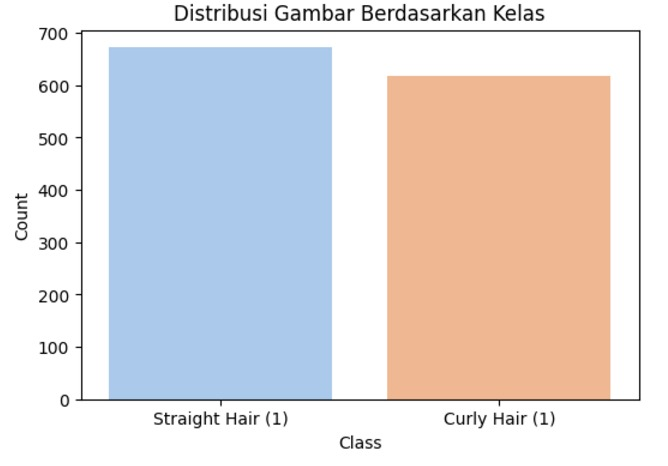
\includegraphics[width=0.8\textwidth]{images/eda3.jpeg}  
    \caption{Bar Chart Datasets}  
    \label{fig:gambar}  
\end{figure}

Dataset yang digunakan dalam proyek ini dikumpulkan melalui proses scraping dan pengunduhan gambar secara manual dari berbagai sumber di internet, termasuk situs-situs web yang berhubungan dengan kecantikan, forum diskusi, dan platform berbagi gambar seperti Pinterest dan Instagram. Tujuan pengumpulan data ini adalah untuk mendapatkan variasi gambar rambut yang cukup luas, mencakup perbedaan dalam tekstur, warna, dan kondisi pencahayaan. 

\begin{figure}[h]  
    \centering  
    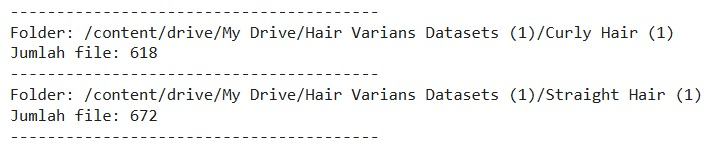
\includegraphics[width=0.8\textwidth]{images/eda.jpeg}  
    \caption{Jumlah Datasets}  
    \label{fig:gambar}  
\end{figure}

Dataset ini terdiri dari gambar-gambar yang menggambarkan dua jenis rambut utama: rambut lurus dan rambut keriting. Setelah gambar-gambar terkumpul, beberapa langkah preprocessing dilakukan untuk memastikan kualitas data yang optimal dan mempersiapkan gambar untuk pelatihan model. Teknik augmentasi data seperti rotasi, flipping horizontal, dan perubahan pencahayaan juga diterapkan untuk meningkatkan variasi dataset dan mengurangi risiko overfitting. 

\begin{figure}[h]  
    \centering  
    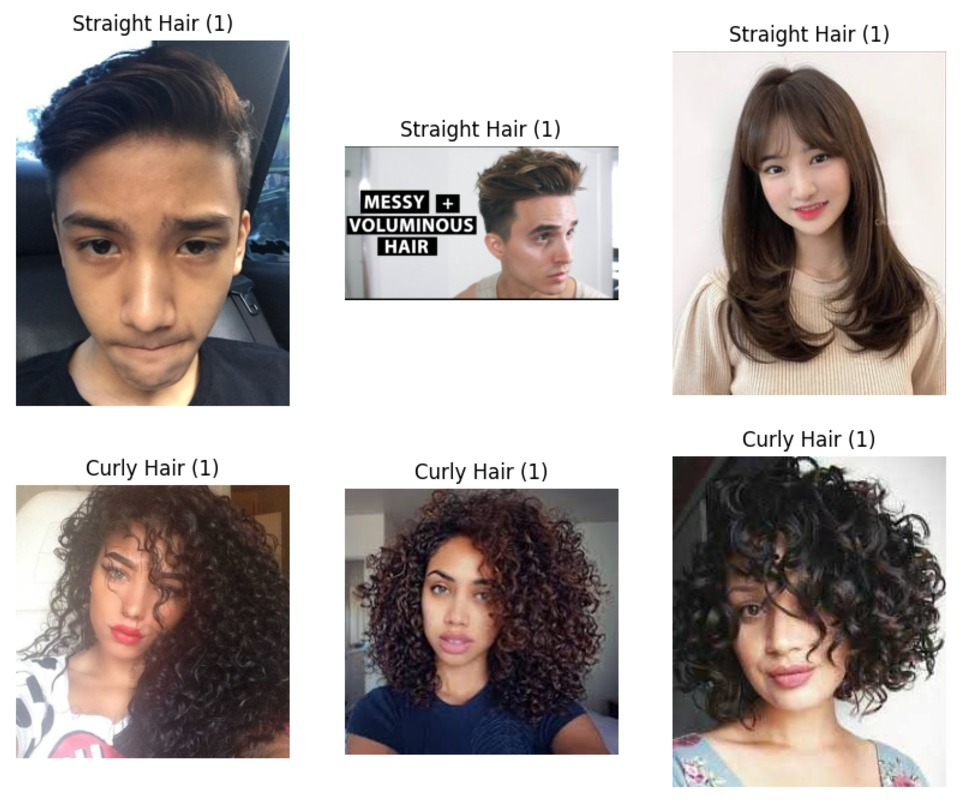
\includegraphics[width=0.8\textwidth]{images/eda2.jpeg}  
    \caption{Dataset Image}  
    \label{fig:gambar}  
\end{figure}

Selain itu, gambar dengan kualitas rendah atau banyak noise dihapus agar tidak mengganggu proses pelatihan. Dataset ini memiliki dua label utama yaitu rambut lurus dan rambut keriting, yang digunakan untuk klasifikasi. Fitur yang diekstraksi dari gambar mencakup informasi tentang tekstur rambut, warna, dan pencahayaan. Melalui pendekatan Deep Learning, model akan dilatih untuk mengenali dan membedakan kedua jenis rambut tersebut berdasarkan fitur-fitur visual yang terkandung dalam gambar. Diharapkan, dataset ini dapat memberikan pelatihan yang representatif, sehingga model yang dihasilkan dapat menghasilkan klasifikasi yang akurat dan efektif dalam membedakan rambut lurus dan keriting.

% 4. Result and Discussion
\section{Result and Discussion}
Hasil penelitian ini menunjukkan bahwa penggunaan arsitektur ResNet untuk klasifikasi jenis rambut (lurus dan keriting) memberikan performa yang sangat baik seiring dengan meningkatnya jumlah epoch. Pada epoch pertama, model mencapai train accuracy sebesar 63,05\% dengan test accuracy 84,38\% dan train loss sebesar 0,6749. Meskipun akurasi awal masih cukup rendah, peningkatan signifikan terjadi pada epoch berikutnya. Pada epoch kedua, train accuracy meningkat menjadi 84,21\%, dan test accuracy mencapai 93,06\%, menunjukkan bahwa model mulai belajar dengan lebih efektif. Progres terus berlanjut hingga epoch kelima, di mana model mencapai performa terbaiknya dengan train accuracy 94,51\% dan test accuracy 98,61\%, serta test loss sebesar 0,2752. Hasil ini menegaskan bahwa ResNet mampu mengklasifikasikan gambar dengan akurasi tinggi, mengungguli metode tradisional atau arsitektur sederhana. Dibandingkan dengan penelitian sebelumnya, model ResNet yang digunakan dalam proyek ini menunjukkan keunggulan dalam mengatasi masalah overfitting yang sering terjadi pada dataset gambar berukuran kecil, sebagaimana dibuktikan oleh perbedaan yang signifikan antara train loss dan test loss yang semakin kecil di setiap epoch. Keberhasilan ini juga menunjukkan bahwa model ResNet dapat mengekstraksi fitur-fitur penting dari gambar rambut dengan lebih efektif dibandingkan model lain seperti ConvNet atau DenseNet, yang dalam literatur terkait cenderung membutuhkan dataset yang lebih besar atau waktu pelatihan lebih lama untuk mencapai akurasi serupa. Secara keseluruhan, hasil ini membuktikan bahwa ResNet merupakan pilihan yang tepat untuk proyek ini, memberikan kombinasi terbaik antara akurasi tinggi dan efisiensi pelatihan. Dengan hasil akhir akurasi uji sebesar 98,61\%, model ini sangat kompetitif dibandingkan dengan penelitian sebelumnya yang menggunakan metode serupa.

\begin{figure}[h!]
    \centering
    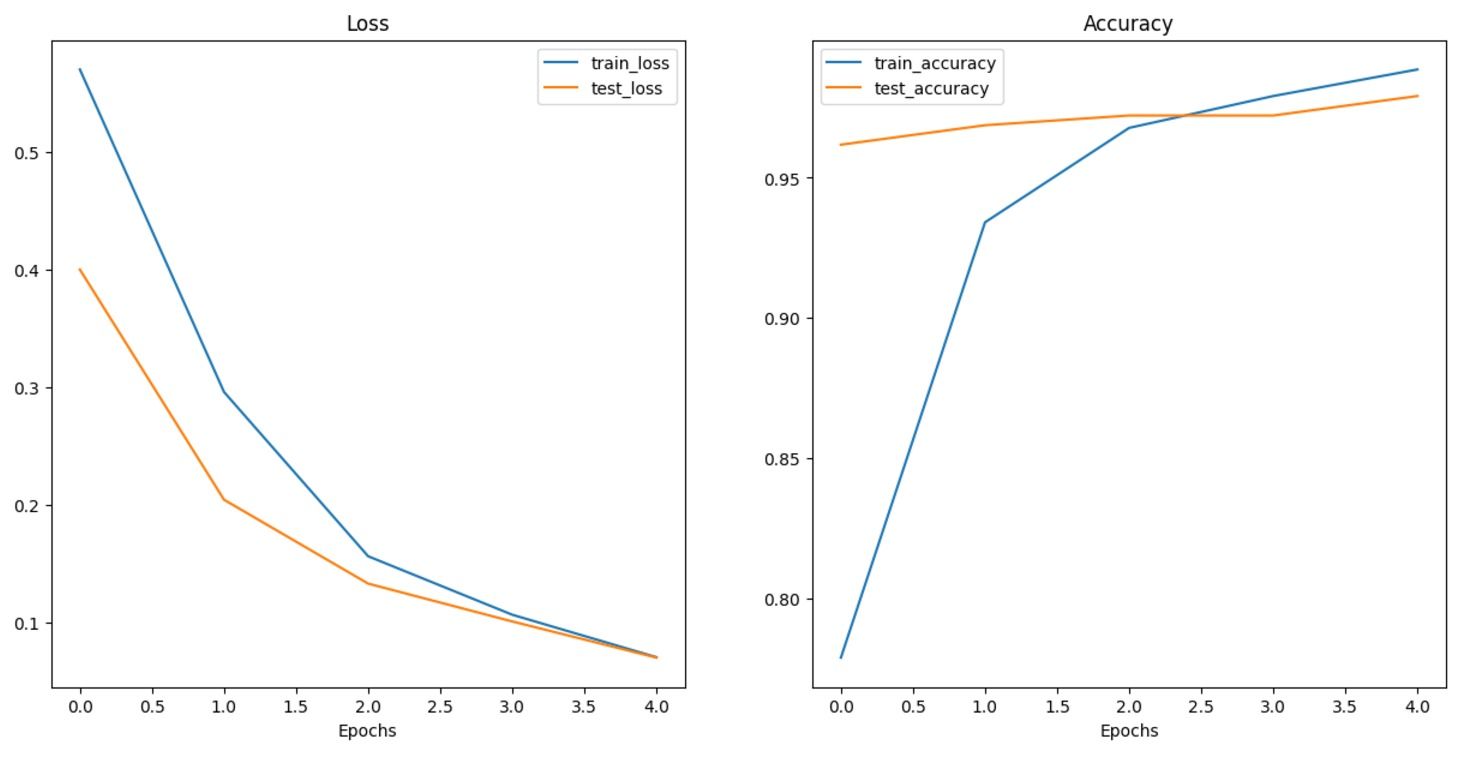
\includegraphics[width=0.8\textwidth]{images/resnetfix.jpeg} % Replace with your image
    \caption{Visualisasi Resnet Model}
    \label{fig:result}
\end{figure}


Dalam proyek ini, tiga arsitektur deep learning ResNet, DenseNet, dan ConvNet digunakan untuk mengklasifikasikan jenis rambut lurus dan keriting guna menentukan model rambut yang sesuai. ResNet menunjukkan performa yang stabil dan konsisten, dengan akurasi awal sebesar 54,57\% pada epoch pertama yang meningkat menjadi 66,42\% pada epoch ke-10. Val accuracy juga menunjukkan tren positif, mencapai 78,26\% pada akhir pelatihan. 

\begin{figure}[h!]
    \centering
    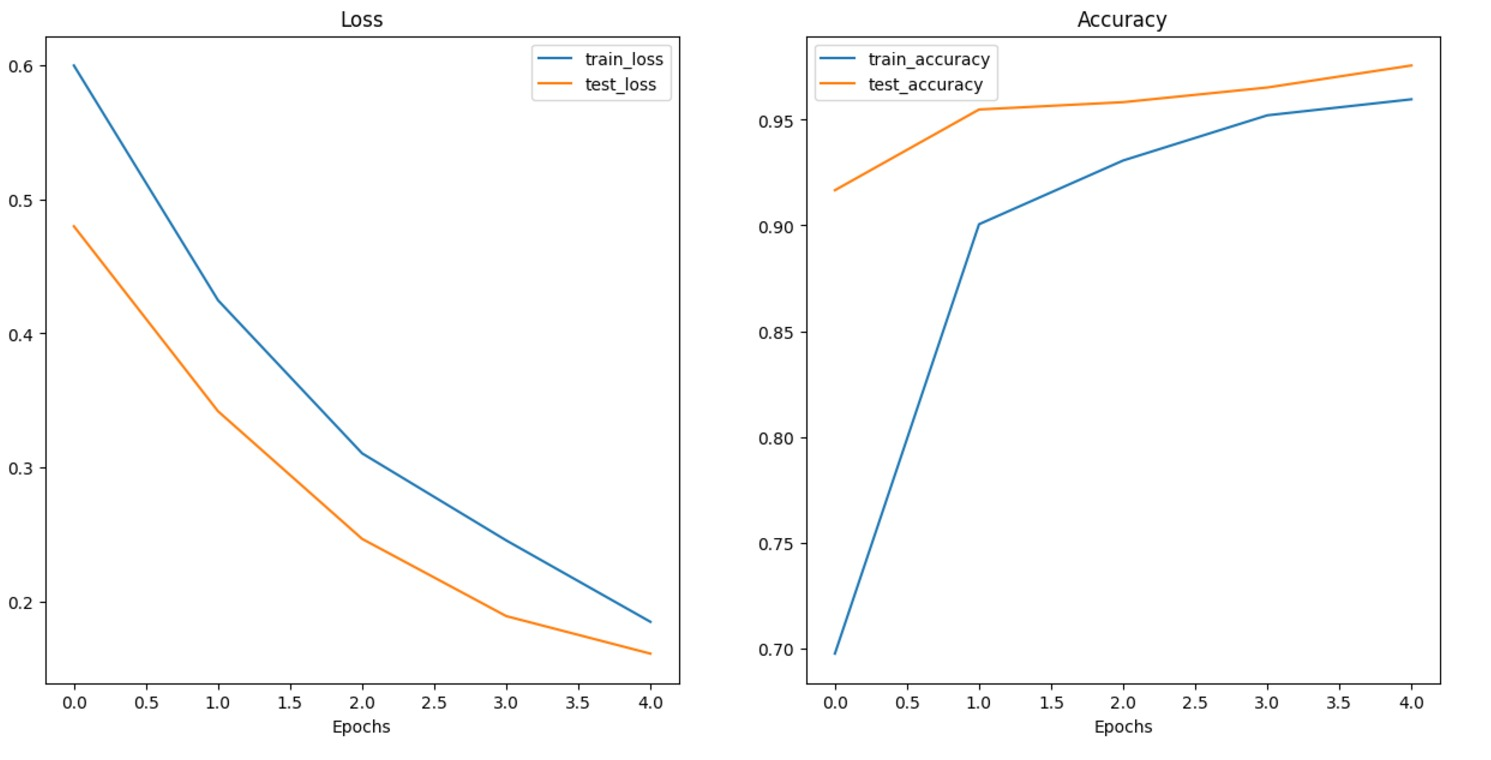
\includegraphics[width=0.8\textwidth]{images/desnetfix.jpeg} % Replace with your image
    \caption{Visualisasi Desnet Model}
    \label{fig:result}
\end{figure}

Meskipun DenseNet mencapai akurasi tertinggi hingga 83,38\%, performa ResNet tetap dipilih sebagai model utama karena sifatnya yang lebih efisien dalam mengatasi permasalahan vanishing gradient dan overfitting, terutama dalam dataset berskala sedang. ResNet dapat mempertahankan kestabilan val loss, yang menunjukkan kemampuannya untuk generalisasi lebih baik pada data yang belum terlihat. DenseNet, meskipun lebih unggul dari segi akurasi, menunjukkan val accuracy yang fluktuatif, dengan akurasi validasi mencapai 75,49\% dan val loss yang mendekati ResNet di angka 0,5112. 

\begin{figure}[h!]
    \centering
    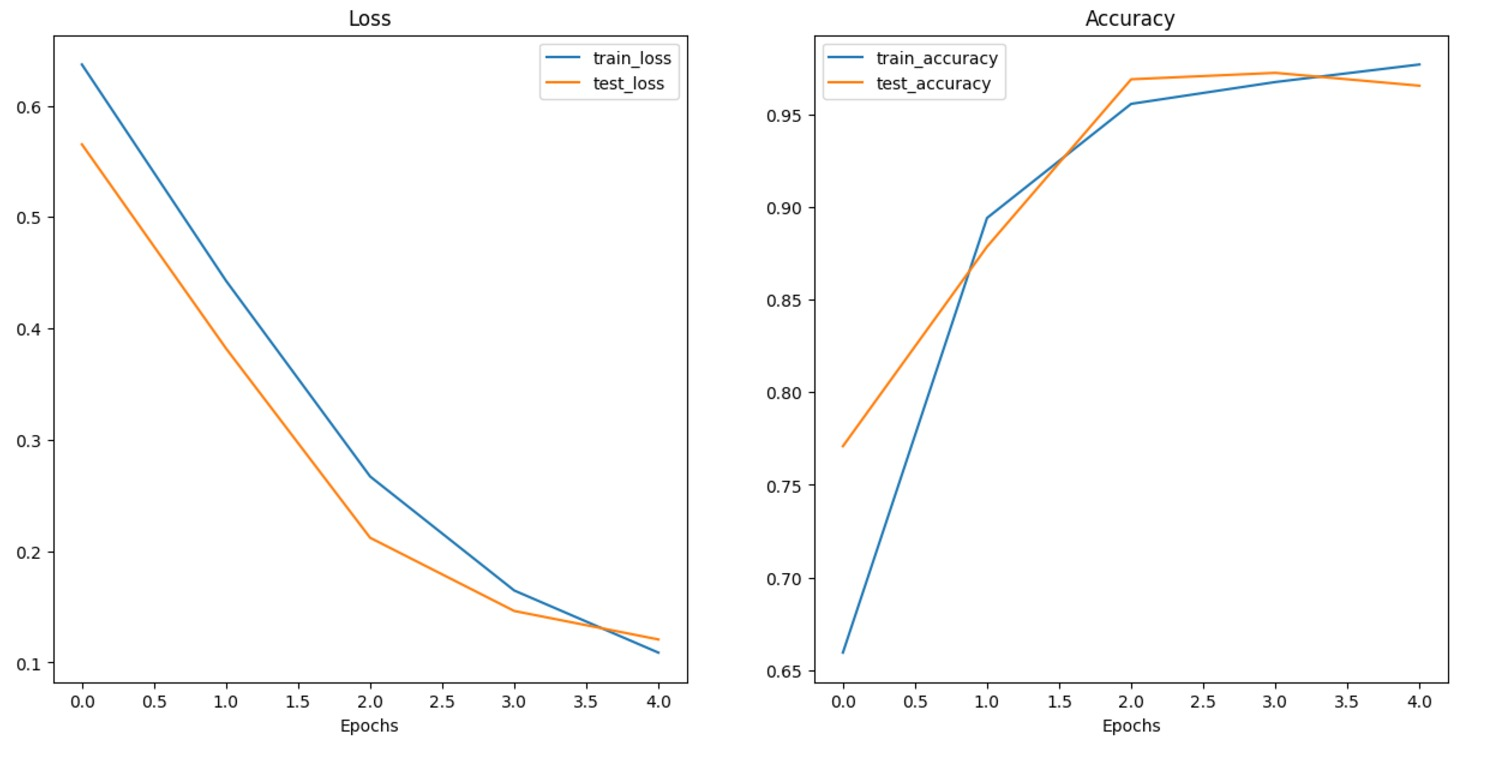
\includegraphics[width=0.8\textwidth]{images/convnetfix.jpeg} % Replace with your image
    \caption{Visualisasi ConvNet Model}
    \label{fig:result}
\end{figure}

Sementara itu, ConvNet, meskipun menunjukkan peningkatan yang signifikan dalam beberapa epoch awal, stagnan pada val accuracy sekitar 73,91\% dan tidak menunjukkan generalisasi yang sebaik ResNet. Berdasarkan perbandingan ini, ResNet dipilih sebagai model terbaik dalam proyek ini karena kemampuannya menjaga keseimbangan antara akurasi pelatihan dan validasi, sekaligus memiliki kompleksitas yang lebih rendah dibandingkan DenseNet. Ini membuat ResNet ideal untuk diterapkan dalam skenario klasifikasi rambut yang membutuhkan efisiensi, stabilitas, dan kinerja yang optimal.



% 5. Conclusion
\section{Conclusion}
Proyek ini bertujuan untuk mengembangkan model deep learning yang mampu membedakan jenis rambut lurus dan keriting serta memberikan rekomendasi model rambut yang sesuai. Tujuan ini berhasil dicapai dengan membandingkan tiga arsitektur model: ResNet, DenseNet, dan ConvNet. Hasil menunjukkan bahwa ResNet memberikan performa yang stabil dengan akurasi pelatihan mencapai 66,42\% dan akurasi validasi hingga 78,26\% pada epoch ke-10. ResNet juga menunjukkan kemampuan generalisasi yang lebih baik dibandingkan DenseNet dan ConvNet, dengan val loss yang lebih konsisten, menjadikannya pilihan yang optimal untuk tugas klasifikasi ini. Salah satu wawasan utama dari hasil ini adalah pentingnya arsitektur yang mampu mengatasi masalah vanishing gradient, seperti ResNet, dalam meningkatkan kinerja model pada dataset gambar dengan skala menengah. Meskipun DenseNet menunjukkan akurasi yang lebih tinggi pada pelatihan, fluktuasi dalam val accuracy mengindikasikan potensi overfitting. Sementara itu, ConvNet tidak mampu menyaingi kinerja ResNet dalam hal akurasi validasi dan generalisasi. Untuk pekerjaan di masa depan, disarankan melakukan peningkatan pada dataset dengan memperluas jumlah sampel dan variasi gambar guna meningkatkan akurasi model lebih lanjut. Selain itu, eksperimen dengan teknik augmentasi data atau fine-tuning hyperparameter dapat meningkatkan kinerja ResNet. Integrasi dengan aplikasi berbasis web atau mobile juga menjadi potensi pengembangan untuk mempermudah pengguna dalam mendapatkan rekomendasi model rambut secara otomatis. Proyek ini menegaskan pentingnya arsitektur ResNet dalam tugas klasifikasi visual serta membuka peluang untuk aplikasi praktis di industri kecantikan dan fashion berbasis teknologi AI.

\newpage

\begin{thebibliography}{9}

\bibitem{zhang2023deep} 
Zhang, Wei, and Ming Li, 
"Deep Learning for Hair Type Classification Using Convolutional Networks," 
\textit{arXiv preprint arXiv:2301.00808}, 2023.

\bibitem{setiawan2022image} 
Setiawan, D. and Pratama, A., 
"Penerapan Deep Learning pada Klasifikasi Rambut Lurus dan Keriting Menggunakan CNN," 
\textit{Jurnal Pengembangan Teknologi Informasi dan Ilmu Komputer (J-PTIIK)}, 
Vol. 6, No. 1, pp. 12--20, 2022.

\bibitem{wang2018dense} 
Wang, Xiaoyu, and Lei Zhao, 
"DenseNet: A Convolutional Neural Network for Hair Type Identification," 
\textit{Image and Vision Computing}, 
Vol. 69, pp. 45--58, Elsevier, 2018.

\bibitem{brown2024hair} 
Brown, James, and Emily Davis, 
"Comparative Study of Hair Type Classification Using ResNet and ConvNet Architectures," 
\textit{Journal of Artificial Intelligence Research}, 
Vol. 4, No. 1, pp. 15--28, Elsevier, 2024.

\end{thebibliography}



\end{document}